\chapter{The Particle Nature of Matter}
    \section{The Atomic Nature of Matter}
        French chemist Lavoisier and his wife, who established the conservation of matter in 
        many careful chemical experiments; \\Dalton, who perceived the atomicity of nature in the law of multiple 
        proportions of compounds; \\Avogadro, who in a most obscure and little-appreciated paper, postulated that 
        all pure gases at the same temperature and pressure have the same number of molecules per unit volume; \\
        and Maxwell, who showed with his molecular-kinetic theory of gases how macroscopic quantities, such as 
        pressure and temperature, could be derived from averages over distributions of molecular properties.\\
        Jean Perrin and the ubiquitous Albert Einstein, who carried on very important theoretical and experimental 
        work concerning Brownian motion, the zigzag movement of small suspended particles caused by molecular impacts.
        Their work produced additional confirmation of the atomic-molecular hypothesis and resulted in improved values of 
        Avogadro’s number as late as the early 1900s.

    \section{The Composition of Atoms}
        There were four major succecful works:
        \begin{itemize}
            \item The discovery of the law of electrolysis in 1833 by Michael Faraday.
            \item The identification of cathode rays as electrons and the measurement of thec harge-to-mass 
            ratio $(e/m_e$) of these particles by Joseph John ( J. J.) Thomson in 1897.
            \item The precise measurement of the electronic charge ($e$) by Robert Millikan in 1909.
            \item The establishment of the nuclear model of the atom by Ernest Rutherford and coworkers Hans Geiger and 
            Ernest Marsden in 1913.
        \end{itemize}

        \begin{wrapfigure}{r}{0.2\linewidth}
            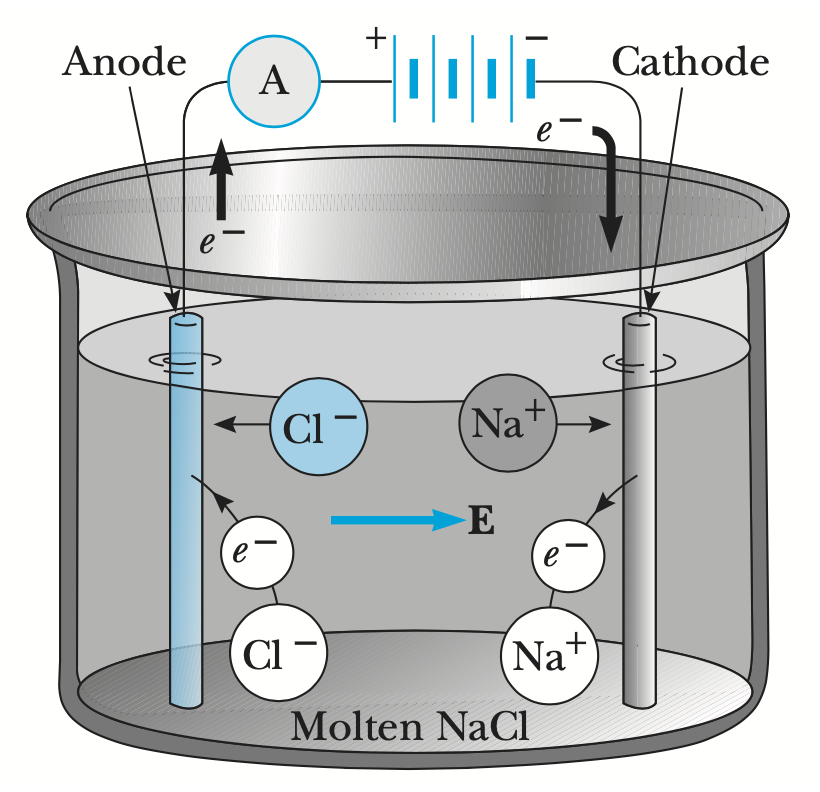
\includegraphics[width=0.9\linewidth]{figures/Electrolysis of molten NaCl.png}
            \caption{Electrolysis of molten NaCl.}
            \label{fig:Electrolysis of molten NaCl}
        \end{wrapfigure}

        \paragraph{Faraday’s Experiment}
        of the electrolysis of molten common salt (NaCl). 
        Faraday found that if \SI{96500}{C} of charge (1 faraday) is passed through such a molten solution, 23.0 g of Na will deposit 
        on the cathode and 35.5 g of chlorine gas will bubble off the anode, see Fig.\eqref{fig:Electrolysis of molten NaCl}. 
        In this case, exactly 1 gram atomic weight 
        or mole of each element is released because both are monovalent. For divalent and trivalent elements, exactly 21 and 13 of 
        a mole, respectively, would be released.

        \paragraph{$\bullet$} Doubling the quantity of charge passed doubles the mass of neutral element freed. Thus 
        \textbf{Faraday’s law of electrolysis}, 
        \coloredeq{eq:Faraday’s law of electrolysis}{m= \frac{q M}{(\num{96500})(valence)}} 
        {\tiny \begin{itemize}
            \item $m$ the mass of the released substance in grams 
            \item $M$ the molar mass in grams
            \item $q$ the total charge passed in coulombs 
        \end{itemize}}

        \paragraph{$\bullet$} Faraday’s law of electrolysis is explained in terms of atoms picture, 
        see Fig.\eqref{fig:Electrolysis of molten NaCl}. Charges passes through the molten solution in form of ions, which they left
        an \textit{excess} or \textit{deficiency} of one or more electrons. By the electric field of the battery, these ions move to
        the anode (where they lose $e^-$) or the cathode (where they gain $e^-$) and are released as neutral elements.

        \starpar Although it was not clear in 1833, Faraday’s law of electrolysis confirmed three important ideas:
        {\small \begin{enumerate}
            \item Matter consists of molecules and that molecules consist of atoms.
            \item Charge is quantized, because only integral numbers of charges are transferred at the electrodes.
            \item The subatomic parts of atoms are positive and negative charges, although they remained unknown.
        \end{enumerate}}

        \paragraph{Joseph John (J. J.)} In 1897, Thomson discovered that the “rays” seen in low-pressure 
        gas discharges were actually caused by negative particles (electrons) ended a debate dating back nearly 30 years:
        Were cathode rays material particles or waves?

        \bulletpar In Thomson's $e/m_e$ experiment, electrons are accelerated from the cathode to the anode, collimated by slits in 
        the anodes, and then allowed to drift into a region of perpendicular electric and magnetic fields.
        The $\vec{E}$ and $\vec{B}$ first are applied to produce an undefflected beam. If the $\vec{B}$ field is then turned off, 
        the beam deflected on the phosphorescent screen. From the deffelctiona and measured values of $\vec{E}$ and $\vec{B}$ the 
        charge-to-mass ratio, $e/m_e$ can be determined.

        \begin{wrapfigure}{r}{0.3\linewidth}
            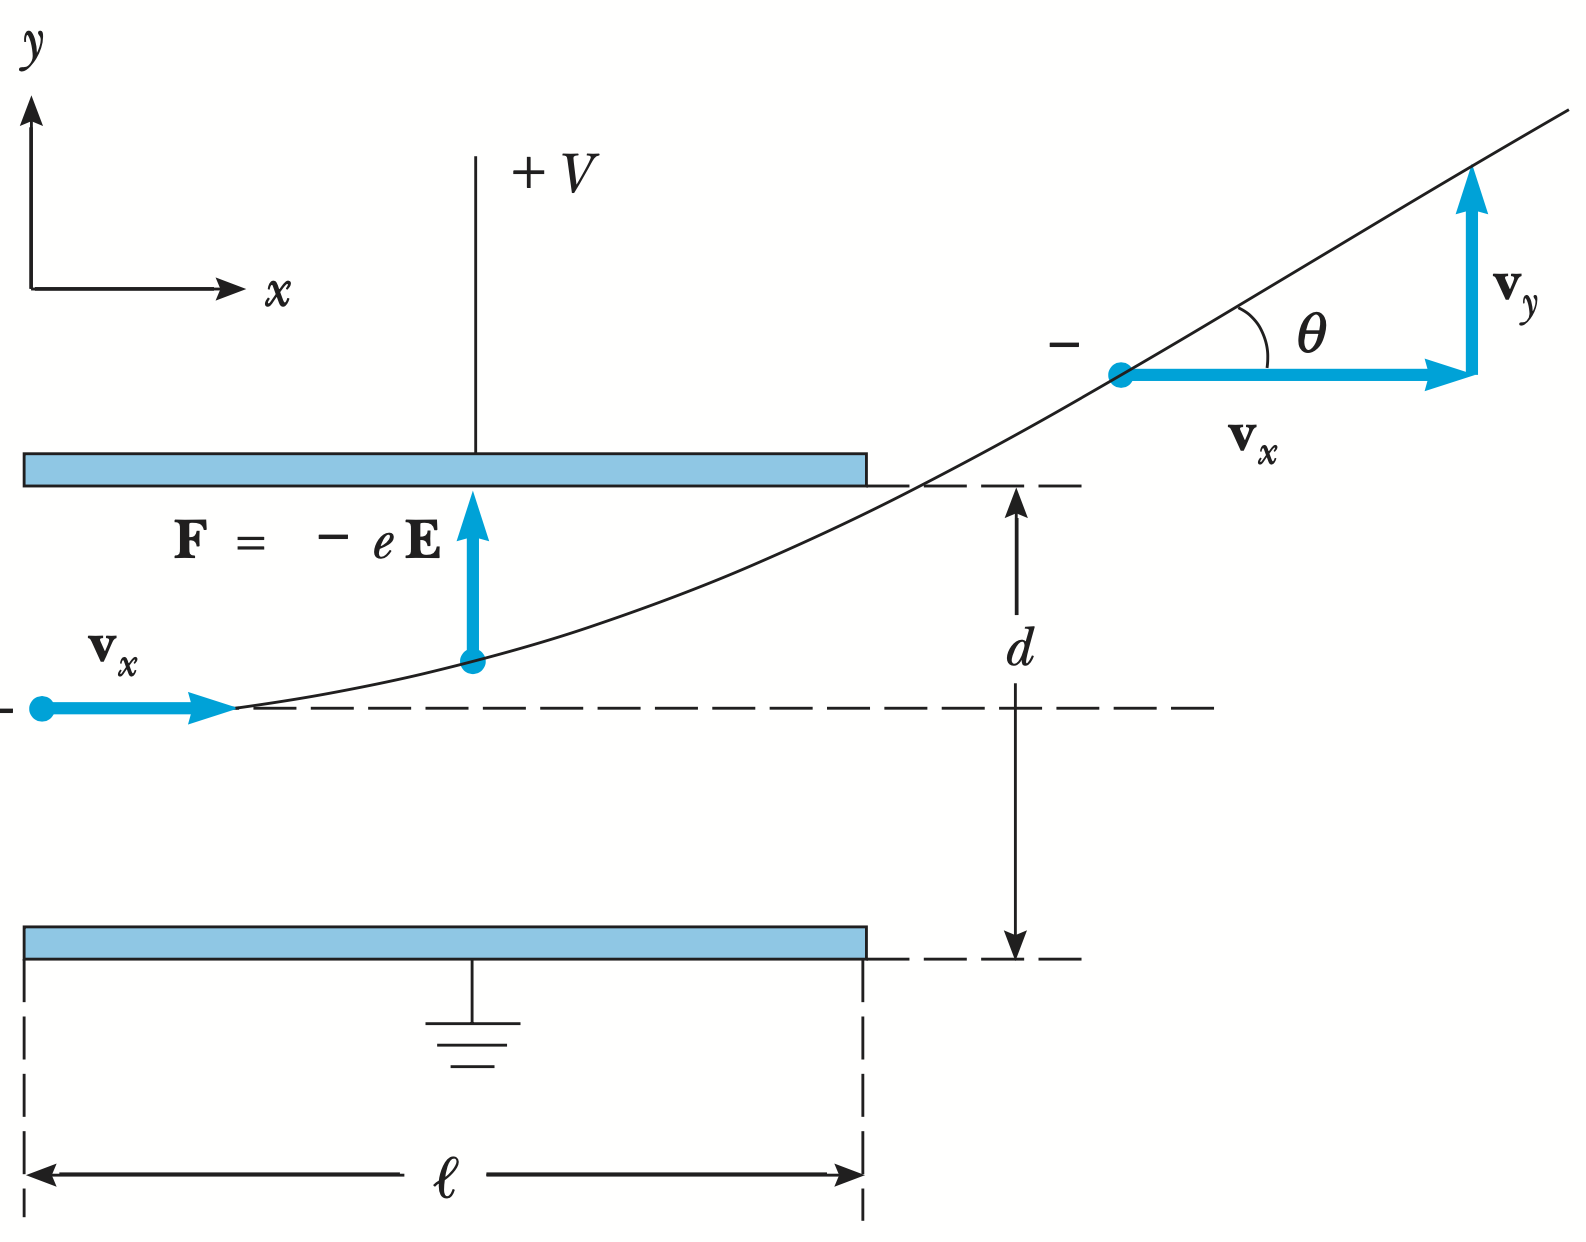
\includegraphics[width=0.9\linewidth]{figures/thomson experiment.png}
            \caption{Defflection of negitve particle}
            \label{fig:defflection path}
        \end{wrapfigure}
        
        \bulletpar In Thomson experiment, see Fig.\eqref{fig:defflection path}, consider when only $\vec{E}$ exists between the plates. 
        $v_x$ remains the constant. $y_x$ is
        constant except between the plates, where the $e^-$ undergoes a constant upward acceleration due to electric force 
        following a parabolic path.

        To solve for the deflection angle, $\lambda$, we must solve for $v_x$ and $v_y$. Because $v_y$ initially is zero, $e^-$ leaves
        the plates with $y$ component velocity given by 
        \begin{align}
            \label{eq:Thomson e/m:1}
            v_y = a_yt
        \end{align}
        We know that $a=F_E/m_e = Ee/m_e = Ve/m_e d$, and $t = \ell/v_x$, where $V$ is the applied voltage. Thus 
        \begin{align}
            \label{eq:Thomson e/m:2}
            v_y = \frac{V e \ell}{m_e d v_x}
        \end{align}
        From Fig.\eqref{fig:defflection path}, $\tan{\theta}= v_y/v_x$ and assuming $\tan{\theta}\approx\theta$, 
        \begin{align}
            \label{eq:Thomson e/m:3}
            \theta \approx \frac{V \ell}{d v_x^2} \left(\frac{e}{m_e}\right)
        \end{align}
        To find $v_x$, Thomson apply a $\vec{B}$ field with exixting $\vec{E}$ field to balance the defflection, then thier forces must
        be equal like
        \begin{align}
            \label{eq:Thomson e/m:4}
            F_E = F_B \Leftrightarrow qE = qv_xB \qquad or \quad v_x = \frac{E}{B} = \frac{V}{Bd}
        \end{align}
        Substituting Eq.\eqref{eq:Thomson e/m:4} into Eq.\eqref{eq:Thomson e/m:3}, 
        \begin{empheq}[box=\fbox]{align}
            \frac{e}{m_e} = \frac{V\theta}{B^2 \ell d}
        \end{empheq}

        \starpar Thomson’s original value was only about \SI{1e11}{C/kg} (accepted value \SI{1.758803e11}{C/kg}), prior experiments 
        on the electrolysis of hydrogen ions had given $q/m$ values for hydrogen of about \SI{e8}{C/kg}. Thus it was clear 
        that Thomson had discovered a particle with a mass about 1000 times smaller than the smallest atom.

        \starpar Thomson noted that the $e/m_e$ ratio was independent of the discharge gas and the cathode metal. Also, 
        the particles emitted when electrical discharges were passed through different gases were found to be the same as 
        those observed in the photoelectric effect. Based on these observations, Thomson concluded that these particles must 
        be a universal constituent of all matter.

        \paragraph{Milikan's Value of the Elementary Charge} % (fold)
        \label{par:Milikan's Value of the Elementary Charge}
        In 1897, Thomson had been unable to determine e or me separately. About two years later, he was close  to the value of $e$ (\SI{1.602e-19}{C}) 
        with values of \SI{2.3e-19}{C} for charges emitted from zinc illuminated by ultraviolet light and \SI{1.1e-19}{C} for charges produced 
        by ionizing x rays and radium emissions. 

        \bulletpar He concluded that “$e$ is the same in magnitude as the charge carried by the 
        hydrogen atom in the electrolysis of solutions.” The technique used by Thomson and his students to measure $e$ is especially 
        interesting because it represents the first use of the \texttt{cloud chamber technique} in physics and also formed the starting point 
        for the famous Millikan oil-drop experiment. 
        
        \bulletpar Charles Wilson, one of Thomson’s students, had discovered that ions act as 
        condensation centers for water droplets when damp air is cooled by a rapid expansion. Thomson used this idea to form charged 
        clouds by using the apparatus.

        $Q$ is the measured total charge of the cloud, $W$ is the measured weight of the cloud, and $v$ is the rate of fall or terminal 
        speed. Thomson assumed that the cloud was composed of spherical droplets having a constant mass (no evaporation) and that 
        the magnitude of the drag force $D$ on a single falling droplet was given by \textbf{Stokes’s law},
        \begin{align}
            \label{eq:Stokes's law}
            D = 6 \pi a \eta v
        \end{align}
        {\tiny \begin{itemize}
            \item $a$ the radius of the droplet
            \item $\eta$ the viscosity of the air
            \item $v$ the terminal speed of the droplet
        \end{itemize}}
        The following procedure was used to find $a$ and $w$, the weight of a single drop. Because $v$ is constant, the droplet is in 
        equilibrium under its weight, $w$, and the drag force, $D$. Hence, we require that $w = D$, or
        \begin{align}
            \label{eq:Stokes's law:1}
            w = D \quad \equiv \quad \frac{4}{3} \pi a^3  \rho g = 6 \pi a \eta v 
            \qquad so \quad 
            a = \sqrt{\frac{9 \eta v}{2 \rho g}}
        \end{align}
        where $\rho$ is the mass density of the droplet. We can find $w$, the weight. 
        Then the number of drops $n$ (or number of ions) is given by $W/w$ and the electronic charge $e$ is equal to $Q/n$, 
        assuming that each droplet carries only \textit{one} electronic charge. This method is inaccurate because the 
        theory applies only to a \textit{single} particle and the particles are all assumed to be \textit{identical} in order to compare 
        the theory to experiments performed on a cloud.

        \bulletpar By observing single droplets Millikan eliminated the problems of assuming all particles to be identical and of making uncertain 
        measurements on a cloud. Millikan’s basic idea was to measure the rate of fall of a single drop acted on by gravity and drag forces, 
        apply Stokes’s law to determine the drop radius and mass, then to measure its upward velocity in an opposing electric field, and 
        hence determine the total charge on an individual drop\footnote{This idea was first applied to charged clouds of water vapor by 
        H. A. Wilson in 1903. Millikan switched from water to oil to avoid problems of a changing droplet mass and radius caused by water 
        evaporation.}.

        \bulletpar Millikan’s experiment is to pass oil droplet charged by an atomizer into a small hole in the upper plate of 
        parallel-capacitor plates. These droplets can be seen against the darkness when they are illuminated. If an $\vec{E}$ field is 
        applied to the capacitor plates, the drop may move slowly upward. A single droplet with constant mass and radius may be followed 
        for hours, alternately \emph{rising} and \emph{falling}, by simply turning the $\vec{E}$ field on and off. 
        The charge is found after a long series of measurements of constant upward velocities one observes a discontinuous change or 
        jump to a different upward velocity (higher or lower). \emph{This discontinuous change is caused by the attraction of an ion to the 
        charged droplet and a consequent change in droplet charge}. Such changes become more frequent when a source of ionizing radiation 
        is placed between the plates.

        \bulletpar The quantitative analysis of the Millikan experiment starts with Newton’s second law applied to the oil drop, 
        $\sigma F_y = ma_y$. Because the drag force $D$ is large, a constant velocity of fall is quickly achieved, and all measurements 
        are made for the case $a_y =0$, or $\sigma F_y =0$. If we assume that the magnitude of the drag force is proportional to the speed 
        ($D = Cv$), and refer to Figure 4.9, we find
        \begin{align*}
            Cv - mg = 0 \qquad \vec{E}\text{ off} \\
            q_1E - mg - C v'_1 = 0 \qquad \vec{E}\text{ on}
        \end{align*}
        Eliminating $C$, 
        \begin{align}
            \label{eq:Millikan's experiment:1}
            q_1 = \frac{mg}{E} \left(\frac{v + v'_1}{v}\right)
        \end{align}
        When the droplet undergoes change in its \emph{upward velocity} from $v'_1$ to $v'_2$ (other remain constant),
        \begin{align}
            \label{eq:Millikan's experiment:2}
            q_2 = \frac{mg}{E} \left(\frac{v + v'_2}{v}\right)
        \end{align}
        Dividing Eq.\eqref{eq:Millikan's experiment:1} by Eq.\eqref{eq:Millikan's experiment:2}
        \begin{empheq}[box=\fbox]{align}
            \frac{q_1}{q_2} = \frac{v+ v'_1}{v + v'_2}
            \label{eq:Millikan's experiment:3}
        \end{empheq}

        \starpar In fact Eq.\eqref{eq:Millikan's experiment:2} is a proof of the quantization of charge, because if successive speed ratios 
        are ratios of \emph{whole} numbers, successive charges on the drop must be multiples of the same elementary charge.

        \bulletpar  To determine the actual value of $e$, we need to find the mass. We can use the droplet radius $a$, from Stokes’s law in
        Eq.\eqref{eq:Stokes's law:1}. Thus the mass is 
        \begin{align*}
            m = \rho \cdot \text{volume} = \rho \frac{4}{3} \pi a^3
        \end{align*}

        \bulletpar Stokes’s law, as Millikan was aware, is only approximately correct for tiny spheres moving through a gas. 
        The expression $D=6 \pi a \eta v$ holds quite accurately for a $\SI{0.1}{cm}$ radius sphere moving through a liquid or for any 
        case where the moving-object radius, $a$, is large compared with the mean free path, $L$, of the surrounding molecules. 
        (The mean free path is essentially the average distance between molecules.) In the Millikan experiment, however, $a$ is of the 
        same order of magnitude as the mean free path of air at STP. Consequently, Stokes’s law overestimates the drag force, because the 
        droplet actually moves for appreciable times through a frictionless “vacuum.” Millikan corrected Stokes’s law by using a drag force 
        whose magnitude is
        \begin{align}
            \label{eq:Corrected Stokes's law}
            D \frac{6 \pi a \eta v}{1 + \alpha (l/a)}
        \end{align}
        and found that $\alpha=\num{0.81}$ gave the most consistent values of $e$ for drops of different radii. Further corrections to Stokes’s 
        law were made by Perrin and Roux.
        % paragraph Milikan's Value of the Elementary Charge (end)

        \paragraph{Rutherford's Model of the Atom} % (fold)
        \label{par:Rutherford's Model of the Atom}
        Ernest Rutherford, and his students Ernest Marsden and Hans Geiger conducted a series of experiments 1909-1914. By noticing a beam of $\alpha$ particles broadened
        on a passing through a metal foil easily penetrated the thin film of metal. Rutherford's apparatus is about: a collimated beam of $\alpha$ particles emitted with 
        speed \SI{2e7}{m/s} hit a thin gold foil. Most of the $\alpha$'s passed straight through the foil, but some were \textit{scattered} at angle $\phi$. The number of 
        scattered $\alpha$'s at each angle per unit detector area and per unit time was measured by aid of a microscope.

        \bulletpar Rutherford's insight was that, the mass and kinetic energy of the $\alpha$'s are large, even for a head-on collision with a particle of mass of a hydrogen
        atom would only deflect the $\alpha$ particle with angle of $1^\circ$!. 

        \bulletpar However the repulsion force on a $\alpha$ particle would much greater the positive charge is assumed to be concentrated at a single point.

        \bulletpar Rutherford assumed that the large-angle scattering is produced by a single nuclear collision and the repulsion dorce is given by Coulomb's law
        \begin{align}
            \label{eq:Coulomb between alpha and nucleus}
            F = k \frac{(2e)(Ze)}{r^2}
        \end{align}
        where $r$ is thr distance between $\alpha$ \& the nucleus, $+2e$ is the charge of $\alpha$, and $Ze$ is the nucleus charge. Rutherford found that the number of 
        $\alpha$ particles entering the detector per unit time, $\Delta{n}$ at an angle $\phi$,
        \begin{align}
            \label{eq:Rutherford number of alpha}
            \Delta{n} = \frac{k^2 Z^2 e^4 N n A}{4R^2 (\frac{1}{2}m_\alpha v_\alpha^2)^2 \sin{\phi/2}^2}
        \end{align}
        {\tiny \begin{itemize}
            \item $R$ distance of the detector and the foil
            \item $\phi$ scattering angle
            \item $N$ number of of nuclei per unit area of the foil
            \item $n$ total number of $\alpha$ particles
            \item $A$ area of the detector
        \end{itemize}}
        Geiger confirmed the dependence of the scattering angle, the foil thinkness, and the $\alpha$ speed.

        \bulletpar Rutherford relized that Eq.\eqref{eq:Coulomb between alpha and nucleus} hold iff the $\alpha$ prticle does not have enough energy to deform of penetrate
        the scattering nucleus, he looked for the threshold where energy $\alpha$ should only just penetrating the nuclear redius at closest approach, so
        \begin{align}
            \label{eq:Rutherford alpha approach}
            \frac{1}{2} m_\alpha v_\alpha^2 = k \frac{(2e)(Ze)}{d_{min}}
        \end{align}
        At high kinetic energy this equation begins to fail. Rutherford confirmed for failure for Eq.\eqref{eq:Rutherford number of alpha} and 
        Eq.\eqref{eq:Rutherford alpha approach} for heavy metals. 

        \starpar As result Rutherford and his students had shown that all the mass and charge of $Ze$ were concentrated in a minute nucleus, and that the electron must 
        circle this nucleus.

        However there new three questions raised: 
        \begin{enumerate}
            \item If in the nucleus only the protons, weher are the other half of the nuclear mass?
            \item What is the force that hold protons in such small distance of \SI{10e-14}{m}?
            \item How do thr electrons move around the nucleus?
        \end{enumerate}
        Rutherford's answer for the first one is that there are additional groupings od neutral particles of electron-proton pair. For the second one, that protons are held
        by an intense electrical force. However, James Chadwick descover it is a very strong force as well as the neutron. The last question was done by Niels Bohr.
        % paragraph Rutherford's Model of the Atom (end)

        \paragraph{The Bohr Atom} % (fold)
        \label{par:The Bohr Atom}
        Recall that glowing solids and liquids (even gases at high densities) emit a continuous distribution of wavelengths. This exhinits  the blackbody radiation curve of
        intensity vs. wavelength.

        \bulletpar In contrast, the discrete line spectrum emitted by low-pressure gas subject to an electric discharge. When light from such setup is examined through
        spectroscope, it is found to consist of a few bright lines.

        \bulletpar Also these lines are a characteristic of a particular element. In 1859, Kirchhoff contributed to spectroscopy, wehre there were the foundation of 
        \textbf{absorption spectroscopy}. Where this explained Joseph Fraunhofer's dark D-lines in the solar spectrum.

        \bulletpar Not all the emission lines are exist in absorption lines. They depend on the temperature and of the absorbing vapor.

        \bulletpar Anders \AA ngstr\"om, meausred the four visible lines of hydrogen atom, while in 1885, Johann J. Balmer found a formula that predict the wavelengths
        of these visible lines: $H_\alpha$ red, $H_\beta$ green, $H_\gamma$ blue, and $H_\sigma$ violet. Balmer's formula is
        \begin{align}
            \label{eq:Balmer formula:1}
            \lambda(cm) = C_2 \left( \frac{n^2}{n^2 - 2^2} \right), \qquad n=3, 4, 5, \dots 
        \end{align}
        where $\lambda$ is the wavelength emitted in $cm$ and $C_2=$\SI{3645.6e-8}{cm}, called the \textbf{convergence limit} because it gaves the wavelength of the line 
        with largest $n$. Today Balmer's formulas is in one single equation 
        \coloredeq{eq:Balmer wavelength formula}{\frac{1}{\lambda} = R \left( \frac{1}{n_f^2} - \frac{1}{n_i^2} \right)}
        where $n_f$ and $n_i$ are integers, and $R$ Rydberg wavelength.
        \begin{table}
            \centering
            \begin{tabular}{c c}
                \hline
                Lyman Seris (uv) & $n_f=1$ \\
                Balmer Seris (vis-uv) & $n_f=2$ \\
                Paschen Seris (IR) & $n_f=3$ \\
                Brackett Seris (IR) & $n_f=4$ \\
                Pfund Seris (IR) & $n_f=5$ \\
                \hline
            \end{tabular}
            \caption{\label{tab:Special Series for the Hydrogen Atom} Special Series for the Hydrogen Atom}
        \end{table}

        \bulletpar Electron revoloving idea around the nucleus has led to a disaster. According Maxwell's theroy, accelerated charges revoloving with orbital frequency $f$
        should radiate light with frequency $f$. As an electron radiate, its oribit radius decreases and its frequency increases, falling into the nucleus. Bohr postulated
        that classical radiation theroy, which had been confirmed by Hertz's experiment, did not hold to atomic-sized systems. He used Plank and Einstein work, where he 
        postulated that: electrons in atoms are generally confined to certain stable, nonradiating energy levels and orbits known as \textbf{stationary states}. He also 
        used Einstein's consept of the photon.

        \paragraph{Assumptions of the Bohr Theory} For an atom of hydrogen:
        \begin{itemize}
            \item The electron moves in circular orbits around the protons unser the influence of the Coulomb force.
            \item Only certain orbits are stabel, where there electrons are not radiate, Hence the energy is fixed and classical mechanics is valid.
            \item Radiation is emitted by the atom when the electron 'jumps' from a higher energatic state to a lower one. This jump cannot be visualized or treated
            \item classically. \textbf{The frequency $f$ of the emitted photon is independent of the electron's orbital motion}. 
            \coloredeq{eq:emitted photon energy}{E_i - E_f = hf}
            \item The size of allowed orbits is determined by an additional quantum condition imposed on the electron's orbital angular momentum; an integer multiple of 
            $\hbar$. \coloredeq{eq:Bohr orbital momentum}{m_e v r = n \hbar, \qquad n=1, 2, 3, \dots}
        \end{itemize}

        Now the total energy of the electeon-proton system is 
        \begin{align}
            \label{eq:Bohr energy:1}
            E = K + U = \frac{1}{2} m_e v^2 - k \frac{e^2}{r}
        \end{align}
        Applying Newton’s second law $F_r = mv^2/r$,
        \begin{align*}
            \frac{k e^2}{r^2} = \frac{m_e v^2}{r}
        \end{align*}
        Thus the kinetic energy 
        \begin{align}
            \label{eq:Bohr energy:2}
            K = \frac{m_e v^2}{2} = \frac{k e^2}{2r}
        \end{align}
        Substituting Eq.\eqref{eq:Bohr energy:2} in Eq.\eqref{eq:Bohr energy:1},
        \begin{align}
            \label{eq:Bohr energy:3}
            E = - \frac{k e^2}{2r}
        \end{align}
        The negative indicate that this is a \textit{bound} electron-proton system.
        We can find the orbits radius from Eq.\eqref{eq:Bohr orbital momentum} and Eq.\eqref{eq:Bohr energy:3},
        \coloredeq{eq:Bhor orbits radii}{r_n = \frac{\hbar^2}{m_e k e^2} n^2, \qquad n=1, 2, 3, \dots} The $r_1$ is called Bhor radius 
        \begin{align*}
            a_0 = \frac{\hbar^2}{m_e k e^2} = \SI{0.529}{\AA}
        \end{align*}

        The quantization of orbits resulted in the quantization of energy, substituting $r_n = n^2 a_0$ in Eq.\eqref{eq:Bohr energy:3},
        \coloredeq{eq:Orbits energy}{
            E_n = - \frac{k e^2}{2 a_0} \left( \frac{1}{n^2} \right)
        }
        $$ E_n = - \frac{\SI{13.6}{eV}}{n^2} $$

        $n$ corresponds to the discrete, or quantized vlues of the atom's energy, called \textbf{quantum numbers}.
        $n=1$ is called the \textbf{ground state}, and $n=2$ is called the \textbf{first excited state}.
        $n= \infty$ and $E = 0$, the electron is removed. The minimum required energy to remove an electron is called \textbf{ionization energy}.
        
        By Eq.\eqref{eq:Orbits energy} and Bohr's third postulate, we can find the wavelength of emitted photon when it jumps, 
        $$ f = \frac{E_i - E_f}{h} $$
        or \coloredeq{eq:Bohr-Balmer wavelength}{\frac{1}{\lambda} = \frac{f}{c} = \frac{k e^2}{2 a_0 h c} \left( \frac{1}{n_f^2} - \frac{1}{n_i^2} \right)}
        This \textit{theretical} result is identical to Balmer's \textit{empirical} formula in Eq.\eqref{eq:Balmer wavelength formula}.

        \bulletpar With this, Bohr explained the apectral series by the electrons trnsitions. He extended his model for hydrogen to other atoms; whose on electron is 
        removed (ionized). Tn general, a single electron orbiting a nucleus of charge $+Ze$, Bohr's theory gives, 
        \begin{align}
            \label{eq:Bohr model other atoms}
            r_n =  \frac{a_0}{Z} n^2, \qquad and \quad E_n = - \frac{ke^2}{2 a_0} \left( \frac{Z^2}{n^2} \right)
        \end{align} 

        Beside all that Bohr explained more in his three-part papaer in 1913:
        \begin{itemize}
            \item He explained why fewer lines are seen unthe absorption hydrogen than  in the emission spectrum.
            \item He explained the emmision of x rays from atoms.
            \item He explained the nuclear origin of $\beta$ particles.
            \item He explained the chemical properties of atoms in terms of the electron shell model.
            \item He explained how atoms associate to form molecules.
        \end{itemize}
        \bulletpar To go deeper, Bohr explained the absorption as the reverse process of emission. Ordinarily, hydrogen are in the ground state ($n=1$), so only the Lyman series 
        will take plce. Balmer series is not seen because the average thermal energy of each atoms is not sufficient to make the electron in the first excited state. 
        That is, the number of electrons in $n=2$ is insufficient in low temperatures.

        \bulletpar Bohr, in his paper part II, attempted to find stabel electronic arrangemnets so that the total angular momentum of all the electrons is quantized and 
        the total energy is minimum. Although this is so difficult when more electrins are introdued in the system, Bohr successed in showing that the hydrogen atom can 
        take another electron to becone an ion $H^-$, and the helium was stable by having a closed inner shell with two electrons. He also, consider the lithium (Z=3), and 
        explained the tendency of lithium to loose the an electron.

        \starpar Bohr's predictions about the multielectron atoms:
        \begin{itemize}
            \item Electrons of elements with higher atomic number form stable concentric \textit{rings}, with definite numbers of electrons allowed for each ring.
            \item The number of electrons in the outter most ring determines the \textit{valency}.
        \end{itemize}
        % paragraph The Bohr Atom (end)


    \section{Bohr's Correspondence Principle; Quantization of Angular Momentum}
        Bohr's Correspondence Principle: \textbf{predictions of quantum theory must correspond to the predictions classical physics in the region of sizes where 
        classical theory is known to hold}.
        For the classical sizes of length, mass, and time, if the quantum number becomes large because if increase size of these quantities, we can say that
        $$ \lim_{n \to \infty}\, [quantum physics] = [classical physics]$$
        This principle becomes a useful tool to test a new quantum results, As Bohr himselfe did to arrive to the consept of the quantized orbital angular momentum.
        Bohr argued that his correspondence principle, the quantum condition for emission ($\Delta{E}=hf$) ans Maxwell's classical radiation theory (accelerated charges 
        with orbital frequency $f$ radiate light with the sane frequency) \textit{must simultaneously hold for the case of the extremely large electronic orbits}.

        \bulletpar Consider two large adjacent orbits $r_1$ and $r_2$,separated with energy $dE$, and orbital angular frequency $\omega$, where the last is approximately
        constant in transition between large orbits. To get know the allowed vslues of the angular momentum from the atom's change in energy, we need a connection 
        bewtween \textit{total energy} of the atom Eq.\eqref{eq:Bohr energy:3}, and the \textit{total momentum} of the atom ($L = m_e v r = m_e \omega r^2$). If the 
        electron is hild by Coulomb force, we can show that
        \begin{align}
            \label{eq:Bohr quantization of L:1}
            \frac{k e^2}{r^2} = \frac{m_e v^2}{r} \quad \Rightarrow\, \frac{1}{r} = \frac{m_e k e^2}{L^2}
            \quad \Rightarrow\, E = - \frac{m_e k^2 e^4}{2 L^2}
        \end{align}
        Taking the derivitive to get the connection bewteen the change in energy and the change in momentum,
        \begin{align}
            \label{eq:Bohr quantization of L:2}
            \frac{dE}{dL} = \frac{m_e k^2 e^4}{L^3}
        \end{align}
        Before let us find $L$ in terms of $\omega$ (electron orbital angular frequency), from Eq.\eqref{eq:Bohr quantization of L:1}
        \begin{align}
            \label{eq:Bohr quantization of L:3}
            L^2 = m_e k e^2 v r \quad \Rightarrow L^3 = (m_e v r) m_e k e^2 r \quad 
            \Rightarrow 
        \end{align}
        Again from Eq.\eqref{eq:Bohr quantization of L:1}
        \begin{align}
            \label{eq:Bohr quantization of L:4}
            ke^2 = m_e v^2 r \quad \Rightarrow\, m_e v r = \frac{k e^2}{v}
        \end{align}
        Substituting in Eq.\eqref{eq:Bohr quantization of L:2}
        \begin{align}
            \label{eq:Bohr quantization of L:5}
            \frac{dE}{dL} = \omega
        \end{align}
        Now consider the enission of a photon of energy $dE = \hbar \omega'$, trnsition from $r_1$ to $r_2$, 
        Eq.\eqref{eq:Bohr quantization of L:5} becomes
        \begin{align}
            \label{eq:Bohr quantization of L:6}
            dE = \omega\,  dL \qquad or \quad \hbar \omega' = \omega\, dL
        \end{align}
        where $\omega'$ is the photon angular frequency, and $\omega$ is the electron orbital frequency. Normally, they are not related, but according the correspondence
        principle for such large orbits, quantum theory must give the same frquency as the Maxwell's law of radiation. Thus, Maxwell's theory requires that 
        the orbital frequency equals to the light frequency, $\omega' = \omega$, hence 
        \begin{align}
            \label{eq:Bohr quantization of L:7}
            \hbar \omega = \omega\, dL \qquad or \quad dL = \hbar
        \end{align}
        Eq.\eqref{eq:Bohr quantization of L:7} shows that the change in the electronic angular momentum for transition between adjacent, large orbits, is \textit{always}
        $\hbar$. Thus, the magintude of total angular momentum of an electron in a orbit is an integer multiple of $\hbar$
        \begin{align}
            \label{eq:Bohr quantization of L:result}
            L = m_e v r = n \hbar
        \end{align}
        Bhor relized that although Eq.\eqref{eq:Bohr quantization of L:result} was derived for large orbits case, it was a universal quantum principle.

    \section{Direct Confirmation of Atomic Energy Levels}
        We saw before the idea of the quantized energy levels in atoms, by observing the the optical line apectra. Howeverm in 1914, a directed experiment was conducted by
        James Franck and Gustav Hertz.

        \begin{wrapfigure}{r}{0.25\linewidth}
            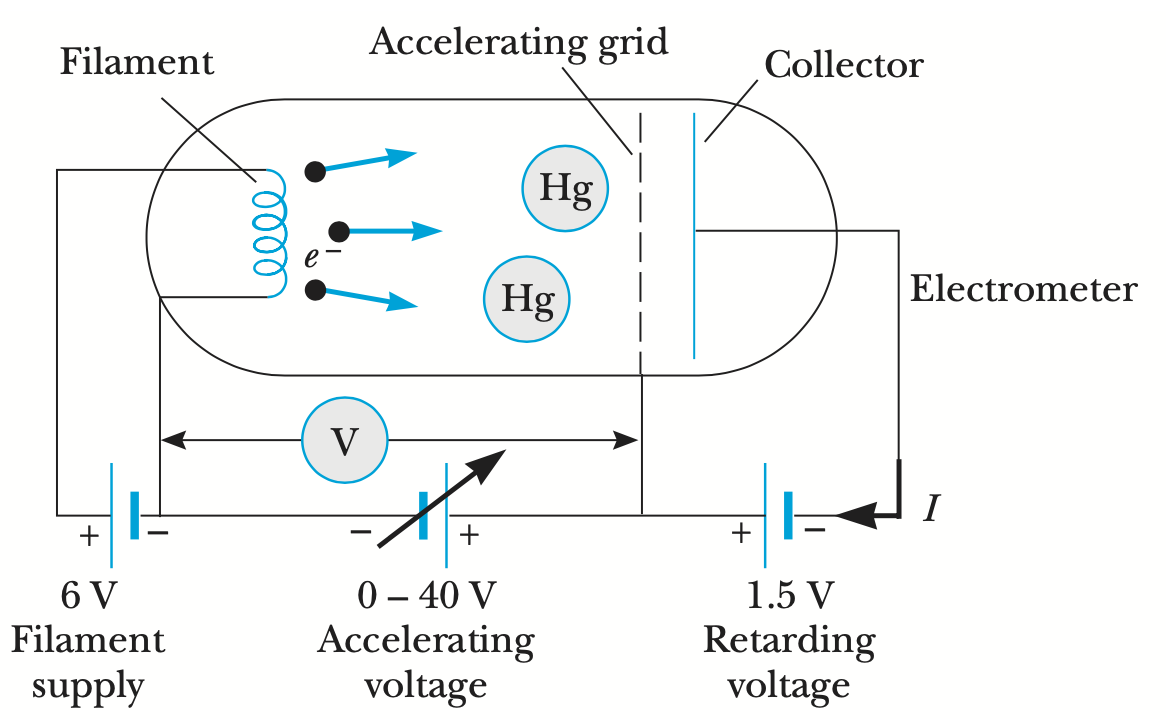
\includegraphics[width=0.9\linewidth]{figures/Franck-Herts apparatus.png}
            \label{fig:Franck-Herts apparatus}
            \caption{Franck-Herts apparatus}
        \end{wrapfigure}

        As in Fig.\eqref{fig:Franck-Herts apparatus}, Franck-Herts apparatus is about electrons emitted by the filament and accelerated throught long regoin 
        ($\approx 1 cm$)by a positive potential on the grid, $V$. The electrons can reach the cllector and be detected by elctrometer (a sensitive ammeter), if they 
        have enough energy to pass potential of 1.5V between the grid and the collector.

        \bulletpar At low electron energies or accelerating voltages, perfectly elastic collisions occur between the electrons and Hg atoms, in which the 
        \textit{sum} of the kinetic energies of electron-atom system is conserved. Since Hg atom is much more massive than the electron, the electron transfers 
        litle KE to the atom. Even with multiple collisions, the electron each the grid with KE of $e \cdot V$.

        \bulletpar As the accelerating voltage is increased, a threshold voltage where the inelastic collisions occur at the grid, with KE$=e \cdot$. In such collisions
        electrons can transfer almost all of thier KE to the atom, raising it to its first excited state. Thus these electrons are unable to overcome the retarding 
        voltage, hence the current $I$ is drop. 
        
        \bulletpar For the second dip in the graph, where $V$ is increased enough so that an electron have two successive inelastic collisions.

        \bulletpar Franck and Hertz with ammeter and voltmeter measurements showed that atoms only accept discrete amounts of energ from electron beam.
        Also, they showed that the enrgy levels obtained from electron bombardment agreed with the spectroscopic results.





